% IEEE conference layout (two-column, Times, 10 pt), set with the standard article class.
\documentclass[10pt,twocolumn,letterpaper]{article}
\usepackage[T1]{fontenc}
\usepackage{mathptmx}
\usepackage[letterpaper,top=0.75in,bottom=1in,left=0.625in,right=0.625in,columnsep=0.25in]{geometry}
\usepackage{amsmath,graphicx,booktabs,tabularx,array,cite,balance}
\usepackage[labelsep=period,font=footnotesize]{caption}
\usepackage{titlesec}
\usepackage{xurl}
\usepackage[hidelinks]{hyperref}
\renewcommand{\thesection}{\Roman{section}}
\renewcommand{\thesubsection}{\Alph{subsection}}
\titleformat{\section}{\centering\normalsize\scshape}{\thesection.}{0.5em}{}
\titleformat{\subsection}{\normalsize\itshape}{\thesubsection.}{0.5em}{}
\titlespacing*{\section}{0pt}{8pt}{4pt}
\titlespacing*{\subsection}{0pt}{6pt}{3pt}
\renewcommand{\thetable}{\Roman{table}}
\DeclareCaptionLabelFormat{ieeetable}{\MakeUppercase{#1}~#2}
\captionsetup[table]{labelformat=ieeetable,labelsep=newline,justification=centering,font={footnotesize,sc}}
\captionsetup[figure]{name=Fig.,labelsep=period}
\setlength{\parindent}{1em}
\setlength{\textfloatsep}{10pt plus 2pt minus 2pt}
\setlength{\dbltextfloatsep}{10pt plus 2pt minus 2pt}
\setlength{\abovecaptionskip}{4pt}
\renewcommand{\topfraction}{0.9}
\renewcommand{\dbltopfraction}{0.9}
\renewcommand{\textfraction}{0.1}
\renewcommand{\floatpagefraction}{0.85}
\pagestyle{plain}
\makeatletter
\renewcommand\@maketitle{%
  \begin{center}
    {\fontsize{21}{25}\selectfont \@title \par}
    \vskip 1em
    {\normalsize \@author \par}
  \end{center}\vskip 1.2em}
\makeatother

\title{Behaviour over Balance: Engagement Profiling, a Relationship Strength Index and Blended Gradient-Boosting Churn Scoring for Customer Retention at a European Bank}
\author{%
\begin{tabular}{c}
Amara Suchitra\\
\textit{Department of Artificial Intelligence and Machine Learning}\\
\textit{Sai Vidya Institute of Technology}\\
Bengaluru, India\\
amarasuchitra@gmail.com
\end{tabular}}
\date{}

\begin{document}
\maketitle

\noindent\textbf{\textit{Abstract}---Inactive customers of a European retail bank leave 1.88 times as often as active ones (26.9\% against 14.3\%), and a large balance does not protect against leaving: customers holding EUR~100,000 or more churn at 25.2\% against 15.9\% for the rest. Using 10,000 customer records from France, Germany and Spain, of whom 20.4\% left, we classify customers into four engagement profiles, measure churn by product count and product mix, and isolate 2,356 inactive high-balance customers whose churn rate is 32.8\%. Product depth protects only up to two products: churn is 27.7\% with one product, 7.6\% with two, and 85.9\% for the 326 customers holding three or four. Credit-card ownership has no significant effect ($p = 0.49$). We combine product fit, activity, tenure and card ownership into a transparent 0--100 Relationship Strength Index whose three tiers churn at 42.1\%, 15.0\% and 5.6\%. A blend of XGBoost, LightGBM and CatBoost is the most accurate of seven models compared (cross-validated AUC 0.869, accuracy 86.6\%) and ranks the customers still at the bank for outreach; we also show that oversampling before splitting, a common practice on this dataset, inflates AUC from 0.830 to 0.923. Bringing inactive premium customers to the churn rate of active ones would retain about 349 customers and EUR~46 million in balances. The results are delivered as an interactive Streamlit dashboard with engagement, product, balance and salary filters.}

\vspace{0.5em}
\noindent\textbf{\textit{Index Terms}---customer churn, retention, customer engagement, product utilisation, cross-selling, relationship strength, gradient boosting, model ensemble, data leakage, banking analytics.}

\section{Introduction}
Keeping an existing customer is usually cheaper than winning a new one, and small gains in retention produce large gains in profit \cite{reichheld,gupta}. Banks therefore invest in churn models \cite{neslin,verbeke,xie}, but most of these models answer \emph{who} will leave and lean on demographics that the bank cannot change. A retention team needs to know which \emph{behaviours} separate customers who stay from those who leave, because behaviours are what a campaign can move.

This work studies churn through engagement and product use. It asks three questions set by the project brief: (1) how strongly is engagement related to churn; (2) does holding more products reduce churn, and is there a limit; and (3) which customers are valuable to the bank yet disengaged, and so likely to leave without warning. Relationship depth is known to matter in financial services \cite{verhoef,vandenpoel,kamakura}; we quantify it for this bank and turn it into a score and a call list.

The contributions are: four engagement profiles with measured churn; evidence that product depth helps only up to two products; evidence that balance is not a loyalty signal and a detector for at-risk premium customers; the five KPIs requested in the brief; a transparent Relationship Strength Index (RSI) with tiers and a threshold; a seven-model benchmark with a leakage test, whose best model ranks outreach; and a deployed dashboard.

\section{Data and Validation}
The European Bank dataset holds one record per customer for 2025: 10,000 customers and 14 fields (Table~\ref{tab:data}). Validation found no missing values and no duplicate customer identifiers. The three binary fields (\textit{HasCrCard}, \textit{IsActiveMember}, \textit{Exited}) contain only 0 and 1, and \textit{NumOfProducts} ranges from 1 to 4. In total 2,037 customers (20.4\%) left. France has 5,014 customers, Germany 2,509 and Spain 2,477. \textit{Year}, \textit{CustomerId} and \textit{Surname} carry no behavioural information and are excluded from modelling.

Two features of the data shape the analysis. First, 3,617 customers (36.2\%) have a zero balance, and none of them is in Germany. Second, the file is a single snapshot: it records whether a customer left, not when, so the analysis shows association and cannot by itself prove cause.

\begin{table}[t]
\caption{Fields Used in the Analysis}\label{tab:data}
\centering\footnotesize
\begin{tabularx}{\columnwidth}{@{}lX@{}}
\toprule
Group & Fields\\
\midrule
Behaviour & NumOfProducts, IsActiveMember, HasCrCard, Tenure\\
Financial & Balance, EstimatedSalary, CreditScore\\
Demographic & Geography, Gender, Age\\
Outcome & Exited (1 = left the bank)\\
\bottomrule
\end{tabularx}
\end{table}

\section{Method}
\subsection{Engagement Profiles}
Each customer is placed in exactly one of four profiles named in the brief: \textit{active engaged} (active, two or more products); \textit{active, low product} (active, one product); \textit{inactive, high balance} (inactive, balance of EUR~100,000 or more); and \textit{inactive disengaged} (inactive, lower balance). The EUR~100,000 premium threshold is close to the lower quartile of funded accounts (EUR~100,182) and can be changed in the dashboard.

\subsection{Key Performance Indicators}
With $c(\cdot)$ the churn rate of a group, the KPIs are: Engagement Retention Ratio $= c(\text{inactive})/c(\text{active})$; Product Depth Index $= (1-c(\text{two products}))/(1-c(\text{one product}))$; High-Balance Disengagement Rate, the share of premium customers who are inactive; Credit Card Stickiness Score $= c(\text{no card}) - c(\text{card})$ in percentage points; and the Relationship Strength Index below. Differences between groups are tested with the chi-square test of independence, and effect size is reported as Cram\'er's $V$. The interval for the small three-or-more-products group uses the Wilson score method \cite{wilson}.

\subsection{Relationship Strength Index}
The RSI is a sum of points, not a fitted model, so that staff can read and explain it:
\begin{equation}
\mathrm{RSI} = P + 30A + 1.5T + 5C,
\end{equation}
where $P$ is product fit (50 for two products, 20 for one, 0 for three or more), $A$ is 1 for an active member, $T$ is tenure in years (0--10) and $C$ is 1 for a credit-card holder. The maximum is 100. Weights follow the evidence in Section~IV: product fit and activity carry the score, while card ownership, which barely moves churn, carries little. Customers are grouped into Weak (0--49), Moderate (50--79) and Strong (80--100) tiers. The index uses no demographic field.

\subsection{Churn Model and Benchmark}
To rank individual customers we compare seven classifiers built with scikit-learn \cite{sklearn}: logistic regression, random forest, gradient boosting \cite{friedman,hastie}, XGBoost \cite{xgboost}, LightGBM \cite{lightgbm}, CatBoost \cite{catboost}, and a blend that averages the probabilities of the last three. All use the same ten fields. Every score is out-of-fold from stratified five-fold cross-validation repeated three times (15 fits per model), so no model is scored on a customer it was trained on. We report the area under the ROC curve (AUC) \cite{fawcett}, accuracy at a 0.5 cut-off, F1 at a cut-off tuned on the other repeats, the number of false alarms, and the expected calibration error (the mean gap between predicted risk and observed churn). Field importance is the loss of out-of-fold AUC when one field is shuffled.

\section{Results}
\subsection{Engagement and Churn}
Inactive members churn at 26.9\% and active members at 14.3\%, an Engagement Retention Ratio of 1.88 ($\chi^2 = 243.0$, $p < 0.001$, $V = 0.16$). Across the four profiles churn runs from 9.7\% for active engaged customers to 32.8\% for inactive high-balance customers (Fig.~\ref{fig:churn}a, Table~\ref{tab:profiles}). The gap between active and inactive customers widens with age (Fig.~\ref{fig:churn}c): among customers aged 51--60, 85.7\% of inactive customers left against 34.7\% of active ones.

\begin{figure*}[t]
\centering
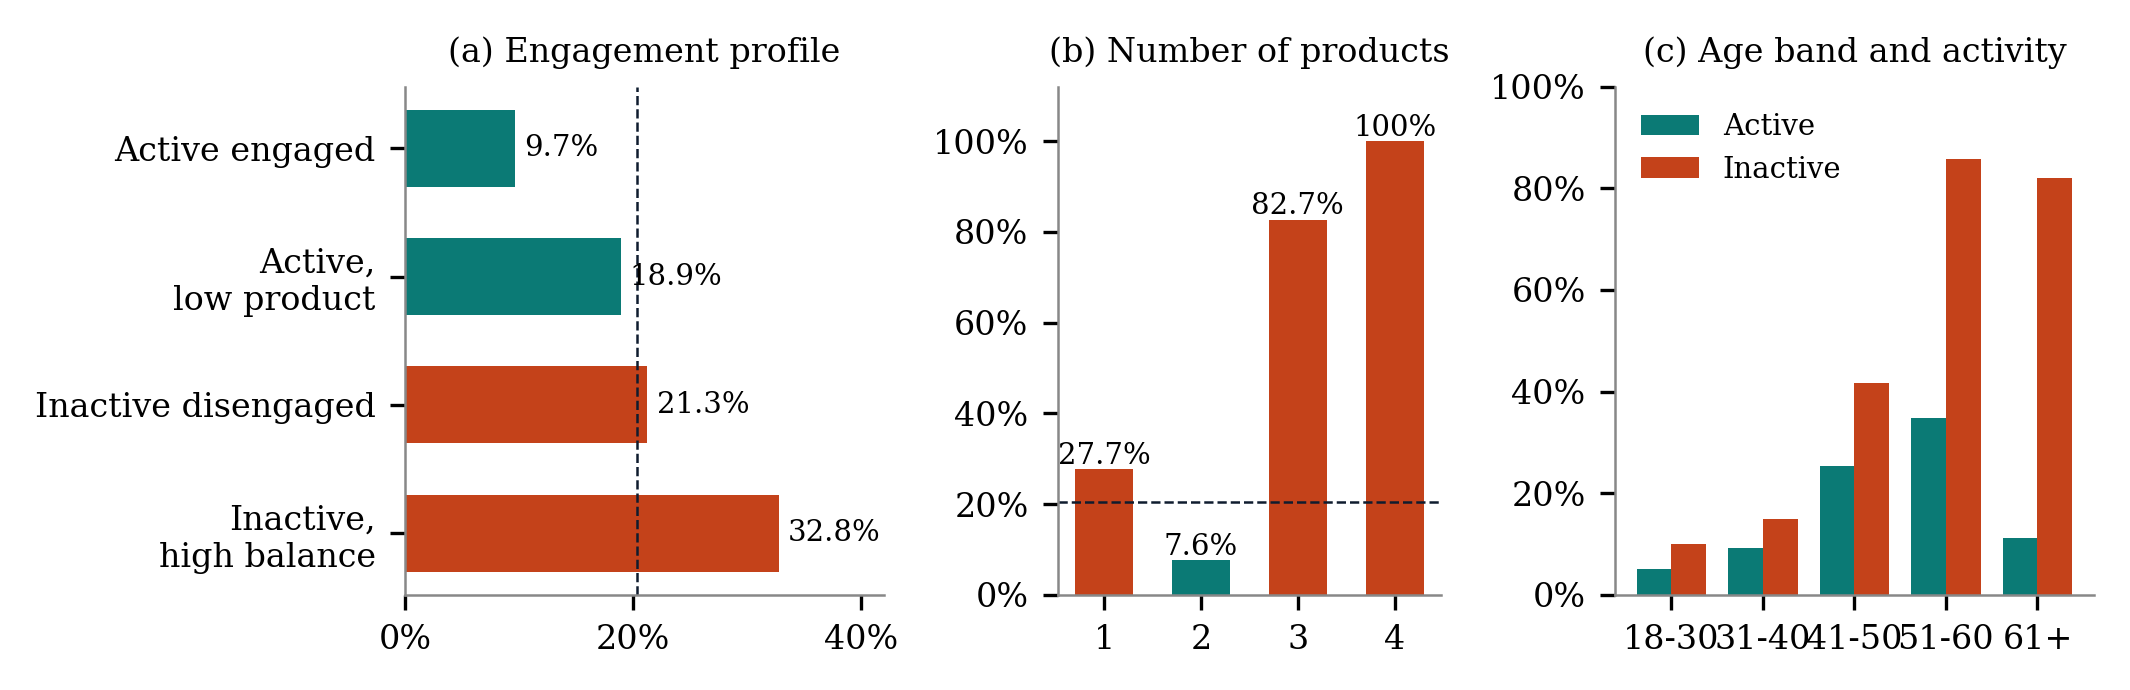
\includegraphics[width=\textwidth]{fig_churn.png}
\caption{Churn rate by (a) engagement profile, (b) number of products and (c) age band and activity. The dashed line is the bank average of 20.4\%.}
\label{fig:churn}
\end{figure*}

\begin{table}[t]
\caption{Engagement Profiles}\label{tab:profiles}
\centering\footnotesize
\begin{tabular}{@{}lrrr@{}}
\toprule
Profile & Customers & Left & Churn\\
\midrule
Active engaged & 2,588 & 250 & 9.7\%\\
Active, low product & 2,563 & 485 & 18.9\%\\
Inactive disengaged & 2,493 & 530 & 21.3\%\\
Inactive, high balance & 2,356 & 772 & 32.8\%\\
\midrule
All customers & 10,000 & 2,037 & 20.4\%\\
\bottomrule
\end{tabular}
\end{table}

\subsection{Product Utilisation}
Product count has the strongest association with churn of any field ($\chi^2 = 1503.6$, $p < 0.001$, $V = 0.39$), but the relationship is not ``more is better'' (Fig.~\ref{fig:churn}b). Churn falls from 27.7\% with one product to 7.6\% with two, a Product Depth Index of 1.28. It then rises to 82.7\% with three products (266 customers) and 100\% with four (60 customers). For the combined group of 326 the rate is 85.9\% (95\% interval 81.7--89.3\%). The group is small, so the exact rate is uncertain, but the direction is not: customers sold a third or fourth product almost all left. The effect of the second product holds in every country; in Germany it takes churn from 42.8\% to 12.1\%.

Activity and product fit add up (Table~\ref{tab:ap}). Active customers with exactly two products are the bank's \emph{sticky} profile: 2,446 customers and 5.6\% churn. Inactive customers with one product churn at 36.7\%.

Credit cards do not make customers stay. Card holders churn at 20.2\% and non-holders at 20.8\%, a Credit Card Stickiness Score of 0.6 points that is not statistically significant ($\chi^2 = 0.5$, $p = 0.49$).

\begin{table}[t]
\caption{Churn by Activity and Product Count}\label{tab:ap}
\centering\footnotesize
\begin{tabular}{@{}lrrrr@{}}
\toprule
 & \multicolumn{2}{c}{Active} & \multicolumn{2}{c}{Inactive}\\
Products & Customers & Churn & Customers & Churn\\
\midrule
1 & 2,563 & 18.9\% & 2,521 & 36.7\%\\
2 & 2,446 & 5.6\% & 2,144 & 9.9\%\\
3 & 113 & 75.2\% & 153 & 88.2\%\\
4 & 29 & 100\% & 31 & 100\%\\
\bottomrule
\end{tabular}
\end{table}

\subsection{Financial Commitment and Engagement}
A high balance is not a loyalty signal. The 4,799 premium customers churn at 25.2\% against 15.9\% for the others ($\chi^2 = 134.0$, $p < 0.001$). Almost half of them are inactive: the High-Balance Disengagement Rate is 49.1\%. These 2,356 \emph{at-risk premium} customers churn at 32.8\%, against 18.0\% for active premium customers (Fig.~\ref{fig:premium}). The 772 who left held EUR~101.6 million; the 1,584 who remain hold EUR~210.6 million.

The premium effect is concentrated in Germany, where every customer has a funded account. Premium customers churn at 35.9\% in Germany and 17.8\% elsewhere, and German inactive premium customers churn at 45.1\% (992 customers). Outside Germany a high balance neither raises churn much nor lowers it. In both cases balance fails to protect, and activity roughly halves churn in every balance and country group.

A salary--balance comparison adds two segments. Customers holding more than twice their annual salary at the bank (1,884) churn at 24.5\%. Customers earning EUR~100,000 or more with an empty account (1,781) churn at only 14.4\%: their main banking is elsewhere, which makes them a growth opportunity more than a retention risk.

\begin{figure}[t]
\centering
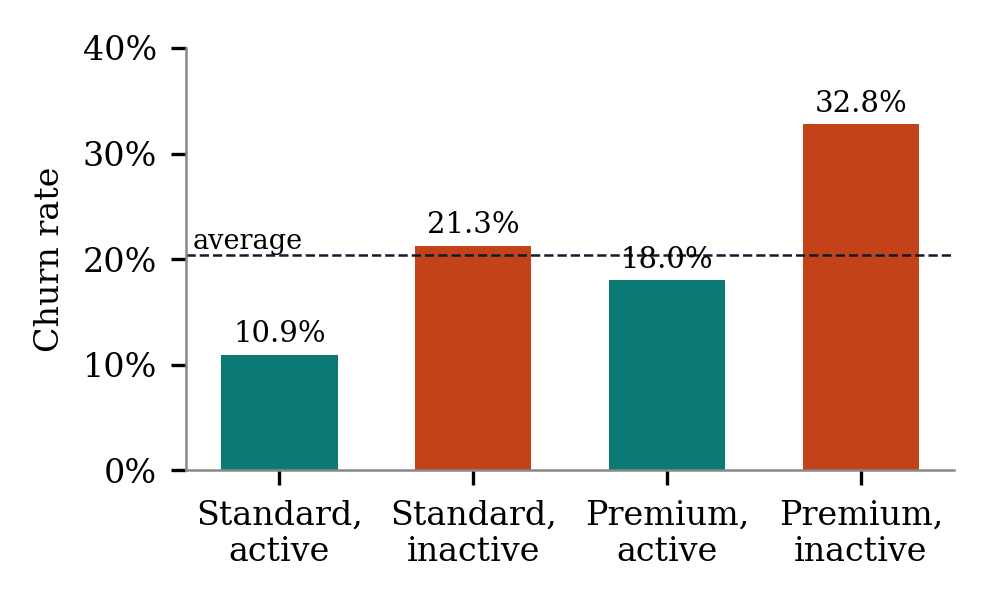
\includegraphics[width=\columnwidth]{fig_premium.png}
\caption{Churn by balance and activity. Premium means a balance of EUR~100,000 or more.}
\label{fig:premium}
\end{figure}

\subsection{Retention Strength}
Customers who stayed have a mean RSI of 63.6 and those who left 44.1. Churn falls across the tiers from 42.1\% to 15.0\% to 5.6\% (Table~\ref{tab:rsi}, Fig.~\ref{fig:rsi}). The engagement threshold is 50: below it 42.1\% of customers leave, at or above it 11.7\%. An inactive single-product customer crosses the threshold with one change, either becoming active or taking a second product. Used alone as a ranking, the RSI gives an AUC of 0.735.

\begin{table}[t]
\caption{Relationship Strength Tiers}\label{tab:rsi}
\centering\footnotesize
\begin{tabular}{@{}lrrrl@{}}
\toprule
Tier & Customers & Left & Churn & Play\\
\midrule
Weak (0--49) & 2,839 & 1,196 & 42.1\% & Save\\
Moderate (50--79) & 4,715 & 705 & 15.0\% & Grow\\
Strong (80--100) & 2,446 & 136 & 5.6\% & Protect\\
\bottomrule
\end{tabular}
\end{table}

\begin{figure}[t]
\centering
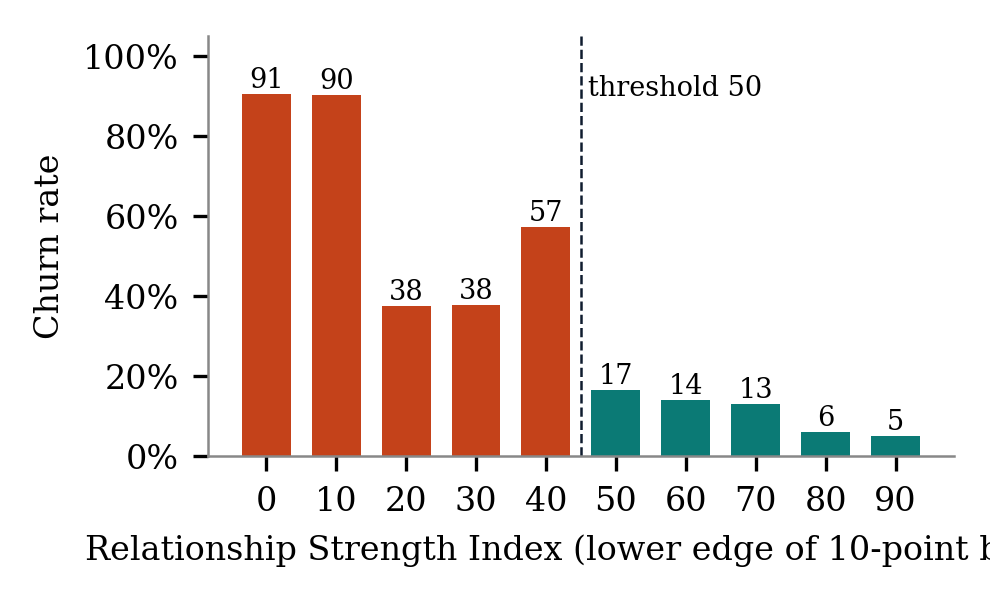
\includegraphics[width=\columnwidth]{fig_rsi.png}
\caption{Churn rate (\%) by Relationship Strength Index band.}
\label{fig:rsi}
\end{figure}

\subsection{Churn Model}
The blend is the most accurate model (Table~\ref{tab:model}): AUC 0.869, accuracy 86.6\% and F1 0.628, with a calibration error of 0.6 points and 313 false alarms among the 7,963 customers who stayed. The four boosted models are close: their AUCs span 0.865--0.869 while the fold-to-fold standard deviation is about 0.006, so the blend is the best choice but not a significant improvement over any one of them. Logistic regression trails at 0.766 because it cannot represent the non-linear effect of product count. Eight engineered features (ratios, flags and interactions) raised logistic regression to 0.840 but did not improve any boosted model. The riskiest 10\% of customers by the blend contain 41.1\% of all churners, and 83.7\% of that decile left.

Product count is the most important field (AUC loss of 0.125 when shuffled), ahead of age (0.116), balance (0.039), activity (0.030) and country (0.028); credit card, tenure, salary and credit score contribute almost nothing. The brief proposes that behaviour, not demographics, drives retention. The data supports a more careful statement: a model using only behaviour fields (AUC 0.772) predicts about as well as one using only demographic fields (0.774), and both are needed for the best result. Age cannot be changed by the bank; product fit and activity can.

\subsection{Why Some Reported Scores Are Higher}
Published accuracy on this dataset is typically 86--87\%, in line with Table~\ref{tab:model}, yet scores above 90\% are often claimed. A frequent cause is applying SMOTE oversampling \cite{smote} before the train--test split, which places synthetic near-copies of test customers in the training data. We reproduced this with a random forest: oversampling before splitting gives an apparent AUC of 0.923 and F1 of 0.85; oversampling inside each training fold, scored on untouched customers, gives 0.830 and 0.57, below the 0.861 of the same model with no oversampling. We therefore use no oversampling and tune the cut-off instead.

\begin{table}[t]
\caption{Model Benchmark (Out-of-Fold, 5-Fold $\times$ 3)}\label{tab:model}
\centering\footnotesize
\begin{tabular}{@{}lrrr@{}}
\toprule
Model & AUC & Accuracy & F1\\
\midrule
Blend (XGBoost + LightGBM + CatBoost) & \textbf{0.869} & \textbf{86.6\%} & 0.628\\
CatBoost & 0.868 & 86.5\% & \textbf{0.630}\\
XGBoost & 0.868 & 86.5\% & 0.626\\
LightGBM & 0.867 & 86.5\% & 0.623\\
Gradient boosting (scikit-learn) & 0.865 & 86.3\% & 0.627\\
Random forest & 0.861 & 86.3\% & 0.622\\
Logistic regression & 0.766 & 81.1\% & 0.493\\
\midrule
Blend, behaviour fields only & 0.772 & & \\
Blend, demographic fields only & 0.774 & & \\
Relationship Strength Index alone & 0.735 & & \\
\bottomrule
\end{tabular}
\end{table}

\section{Dashboard}
The findings are delivered as a Streamlit web application with five views: engagement against churn; product utilisation; a high-value disengaged customer detector; relationship strength scoring; and recommendations. Filters for engagement, country, product count, minimum balance, minimum salary, age and card ownership apply to every view, and every figure recalculates from the customers in view. The detector has an adjustable premium threshold and lists the inactive premium customers still at the bank, ranked by the blended model's risk, each with a suggested action; the list can be downloaded. A calculator shows how a customer's RSI and tier change when a behaviour changes.

\section{Recommendations}
\textit{1) Contact inactive premium customers first, starting in Germany.} If the 2,356 inactive premium customers churned at the rate of active premium customers (18.0\% instead of 32.8\%), about 349 more would stay, holding roughly EUR~46 million. This is an upper estimate that assumes reactivation carries the full effect of being active.

\textit{2) Make the second product the standard bundle.} The 2,078 active single-product customers still at the bank are the easiest cross-sell.

\textit{3) Do not sell past two products without review.} Examine how the 326 three- and four-product relationships were sold before repeating the pattern.

\textit{4) Assign relationship managers to inactive customers aged 51--60,} where inactivity raises churn from 34.7\% to 85.7\%.

\textit{5) Do not rely on credit cards as a loyalty tool.}

\section{Limitations}
The data is one snapshot without dates, so it shows association, not cause: inactivity may be an early stage of leaving as much as a reason for it, and the three-or-more-products pattern may reflect a last attempt to keep customers already leaving. \textit{IsActiveMember} is a single yes/no flag with no detail on what activity means. Product type is unknown; only the count is recorded, so product \emph{mix} can be studied only through count and card ownership. RSI weights were set by judgement from the same data they are evaluated on. The retained-balance estimate is a scenario, not a forecast, and should be tested with a controlled campaign.

\section{Conclusion}
For this bank, how customers use the bank separates leavers from stayers at least as well as who they are. Activity roughly halves churn, two products is the point of greatest loyalty, more than two is a warning sign, and a large balance offers no protection. A transparent Relationship Strength Index and a leakage-free blended churn model turn these findings into a ranked call list that a retention team can act on today.

\balance
\begin{thebibliography}{00}\footnotesize
\bibitem{reichheld} F. F. Reichheld and W. E. Sasser, ``Zero defections: Quality comes to services,'' \textit{Harvard Bus. Rev.}, vol. 68, no. 5, pp. 105--111, 1990.
\bibitem{gupta} S. Gupta, D. R. Lehmann, and J. A. Stuart, ``Valuing customers,'' \textit{J. Marketing Res.}, vol. 41, no. 1, pp. 7--18, 2004.
\bibitem{neslin} S. A. Neslin, S. Gupta, W. Kamakura, J. Lu, and C. H. Mason, ``Defection detection: Measuring and understanding the predictive accuracy of customer churn models,'' \textit{J. Marketing Res.}, vol. 43, no. 2, pp. 204--211, 2006.
\bibitem{verbeke} W. Verbeke, K. Dejaeger, D. Martens, J. Hur, and B. Baesens, ``New insights into churn prediction in the telecommunication sector: A profit driven data mining approach,'' \textit{Eur. J. Oper. Res.}, vol. 218, no. 1, pp. 211--229, 2012.
\bibitem{xie} Y. Xie, X. Li, E. W. T. Ngai, and W. Ying, ``Customer churn prediction using improved balanced random forests,'' \textit{Expert Syst. Appl.}, vol. 36, no. 3, pp. 5445--5449, 2009.
\bibitem{verhoef} P. C. Verhoef, ``Understanding the effect of customer relationship management efforts on customer retention and customer share development,'' \textit{J. Marketing}, vol. 67, no. 4, pp. 30--45, 2003.
\bibitem{vandenpoel} D. Van den Poel and B. Larivi\`ere, ``Customer attrition analysis for financial services using proportional hazard models,'' \textit{Eur. J. Oper. Res.}, vol. 157, no. 1, pp. 196--217, 2004.
\bibitem{kamakura} W. A. Kamakura, S. N. Ramaswami, and R. K. Srivastava, ``Applying latent trait analysis in the evaluation of prospects for cross-selling of financial services,'' \textit{Int. J. Res. Marketing}, vol. 8, no. 4, pp. 329--349, 1991.
\bibitem{wilson} E. B. Wilson, ``Probable inference, the law of succession, and statistical inference,'' \textit{J. Amer. Statist. Assoc.}, vol. 22, no. 158, pp. 209--212, 1927.
\bibitem{friedman} J. H. Friedman, ``Greedy function approximation: A gradient boosting machine,'' \textit{Ann. Statist.}, vol. 29, no. 5, pp. 1189--1232, 2001.
\bibitem{hastie} T. Hastie, R. Tibshirani, and J. Friedman, \textit{The Elements of Statistical Learning: Data Mining, Inference, and Prediction}, 2nd ed. New York, NY, USA: Springer, 2009.
\bibitem{sklearn} F. Pedregosa \textit{et al.}, ``Scikit-learn: Machine learning in Python,'' \textit{J. Mach. Learn. Res.}, vol. 12, pp. 2825--2830, 2011.
\bibitem{xgboost} T. Chen and C. Guestrin, ``XGBoost: A scalable tree boosting system,'' in \textit{Proc. 22nd ACM SIGKDD Int. Conf. Knowl. Discovery Data Mining}, 2016, pp. 785--794.
\bibitem{lightgbm} G. Ke \textit{et al.}, ``LightGBM: A highly efficient gradient boosting decision tree,'' in \textit{Adv. Neural Inf. Process. Syst.}, vol. 30, 2017, pp. 3146--3154.
\bibitem{catboost} L. Prokhorenkova, G. Gusev, A. Vorobev, A. V. Dorogush, and A. Gulin, ``CatBoost: Unbiased boosting with categorical features,'' in \textit{Adv. Neural Inf. Process. Syst.}, vol. 31, 2018.
\bibitem{smote} N. V. Chawla, K. W. Bowyer, L. O. Hall, and W. P. Kegelmeyer, ``SMOTE: Synthetic minority over-sampling technique,'' \textit{J. Artif. Intell. Res.}, vol. 16, pp. 321--357, 2002.
\bibitem{fawcett} T. Fawcett, ``An introduction to ROC analysis,'' \textit{Pattern Recognit. Lett.}, vol. 27, no. 8, pp. 861--874, 2006.
\end{thebibliography}
\end{document}
